\chapter{Predpoklady merania} \label{ch:meranie}



\lettrine{V}{ praktických} aplikáciach sa vyskytuje takmer výhradne indukčná záťaž, preto je aj táto práca zameraná na meranie takejto záťaže. Indukčnosťou zabezpečený v krátkom čase $t_{on}$, $t_{off}$ konštantný prúd $I_L$ navyše umožňuje prehľadnú analýzu zmeraných priebehov.

Meranie bude vykonávané na tranzistorovom spínači s napäťovým medziobvodom podľa Obr. \ref{fig:schema_zakladna}
\begin{figure}[!ht]
	\centering
	% XCircuit output "schema_zakladna.tex" for LaTeX input from schema_zakladna.ps
\def\putbox#1#2#3#4{\makebox[0in][l]{\makebox[#1][l]{}\raisebox{\baselineskip}[0in][0in]{\raisebox{#2}[0in][0in]{\scalebox{#3}{#4}}}}}
\def\rightbox#1{\makebox[0in][r]{#1}}
\def\centbox#1{\makebox[0in]{#1}}
\def\topbox#1{\raisebox{-0.60\baselineskip}[0in][0in]{#1}}
\def\midbox#1{\raisebox{-0.20\baselineskip}[0in][0in]{#1}}
   \scalebox{0.8}{
   \normalsize
   \parbox{2.60335in}{
   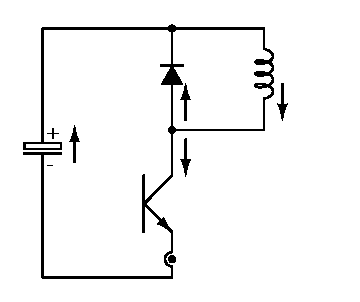
\includegraphics[scale=1.25]{schema_zakladna}\\
   % translate x=284 y=237 scale 0.28
   \putbox{1.45in}{0.99in}{1.20}{\llgic}%
   \putbox{1.45in}{1.49in}{1.20}{\llgiD}%
   \putbox{2.26in}{1.45in}{1.20}{\llgiL}%
   \putbox{0.52in}{1.14in}{1.20}{\llgiK}%
   } % close 'parbox'
   } % close 'scalebox'
   \vspace{-\baselineskip} % this is not necessary, but looks better

	\caption{Tranzistorový spínač s napäťovým medziobvodom a indukčnou záťažou}
	\label{fig:schema_zakladna}
\end{figure}

Napäťové priebehy budú snímané priamo napäťovou sondou širokopásmového osciloskopu, prúd tranzistorom bude snímaný snímačom prúdu, bližšie popísaným v stati \ref{sec:snimanie_prudu}.
Vzhľadom na vysoké frekvenčné pásmo je nutné výstup zo snímača resp. vstup do osciloskopu impedančne prispôsobiť s koaxiálnym káblom (sondy osciloskopu). %Tomuto problému je venovaný Dodatok \ref{ch:priloha_vedenie}.

V snahe o hodnoverné zmeranie priebehov charakteristických pre konkrétnu súčiastku  je nutné eliminovať vplyvy (obzvlášť tie, ktoré nemožno presne identifikovať) ostatných prvkov, ktorými sú hlavne:
\begin{itemize}
	\item kapacita obvodu do okolia (do zeme), spôsobujúca unikajúce impulzné prúdy. V prípade úniku cez tieniaci vodič koaxiálneho kábla vzniká na jeho indukčnosti a odpore úbytok, ktorý sa pripočítavá k skutočnému snímanému signálu. Kvôli obmedzeniu kapacity bude celé meracie pracovisko v dobe merania odpojené od siete - medziobvod bude tvoriť nabitá kondenzátorová batéria, osciloskop bude napájaný akumulátorom a budič monočlánkami. Prenos riadiaceho signálu z generátora je realizovaný optickým vláknom s minimálnou kapacitou.
	\item indukčnosť v slučke medziobvod - tranzistor - dioda, spôsobujúca prekmity a úbytky v priebehoch. Pre obmedzenie indukčnosti je výhodné radiť väčšie množstvo kondenzátorov v medziobvode paralelne a prepojenie s tranzistorom realizovať sendvičovým spojom.
	\item nulová dioda, deformujúca priebehy zotavovacími dejmi. Pre minimalizovanie vplyvu diody budú vyberané diody rýchlejšie od tranzistora.
\end{itemize}


Meranie bude vykonané metódou \uv{double shot}, tj. dvomi pulzmi, počas ktorých postupne narastá prúd tlmivkou. Šírka pulzov a indukčnosť tlmivky určujú veľkosť prúdu v čase zapínania a vypínania tranzistora.

\myfig{schema_pracovisko}{Usporiadanie meracieho pracoviska.}{\label{fig:schema_pracovisko}}

Usporiadanie meracieho pracoviska je schematicky znázornené na Obr. \ref{fig:schema_pracovisko}

\section{Umiestnenie meracej zeme} \label{sec:umiestnenie_meracej_zeme}
Spoločná meracia zem sónd osciloskopu musí byť realizovaná tak, aby spoločný potenciál jednotlivých pripojení zemí bol skutočne spoločný aj pri rýchlych dynamických dejoch. Navyše je prirodzená potreba, aby sa na tomto potenciále nachádzal emitor tranzistora (čipu vo vnútri púzdra). Dynamický rozdiel potenciálov galvanicky spojených bodov je spôsobovaný indukčnosťou tohto spojenia. Preto musia byť zeme sónd pripojené geometricky v zhodnom bode, a tento musí byť umiestnený čo najbližšie k emitoru čipu. Vývody púzdra ako aj zapúzdrené bondovacie dráty zďaleka nemajú zanedbateľnú indukčnosť, ako bude overené aj meraním (kapitola \ref{ch:vysledky}). Na výkonovom emitorovom prívode vznikajú veľké hodnoty $\dif{i}/\dif{t}$, čím sa jeho indukčnosť neodstrániteľne prejaví úbytkom napätia, čo je najmä v prípade súčiastok bez vyvedeného riadiaceho emitoru (nielen) z hľadiska umiestnenia meracej a v aplikáciách hlavne riadiacej zeme značne nevýhodné.


\begin{figure}[!ht]
	\centering
	% XCircuit output "priebehy_1.tex" for LaTeX input from priebehy_1.ps
\def\putbox#1#2#3#4{\makebox[0in][l]{\makebox[#1][l]{}\raisebox{\baselineskip}[0in][0in]{\raisebox{#2}[0in][0in]{\scalebox{#3}{#4}}}}}
\def\rightbox#1{\makebox[0in][r]{#1}}
\def\centbox#1{\makebox[0in]{#1}}
\def\topbox#1{\raisebox{-0.60\baselineskip}[0in][0in]{#1}}
\def\midbox#1{\raisebox{-0.20\baselineskip}[0in][0in]{#1}}
   \scalebox{0.8}{
   \normalsize
   \parbox{4.44792in}{
   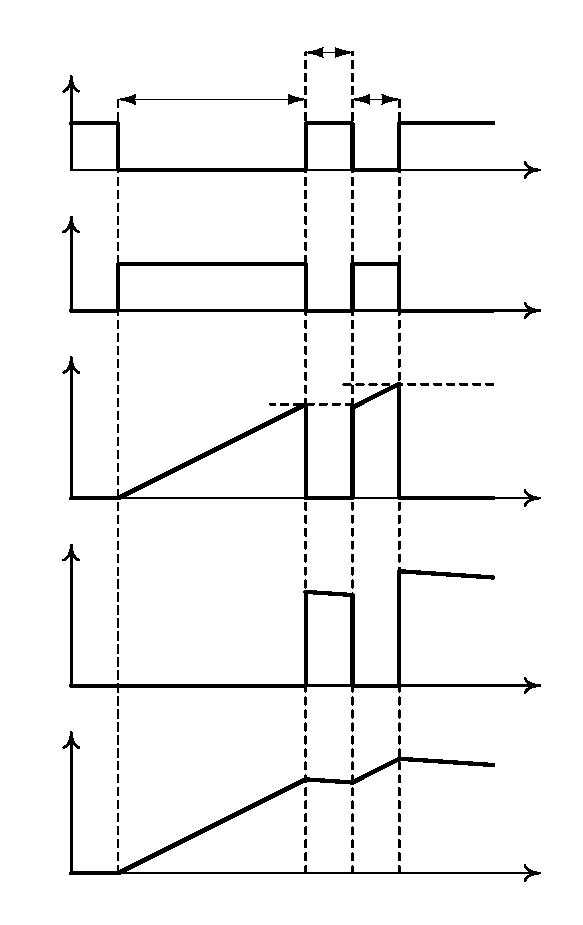
\includegraphics[scale=1.25]{priebehy_1}\\
   % translate x=314 y=1408 scale 0.30
   \putbox{4.17in}{4.78in}{1.20}{\llgt}%
   \putbox{0.06in}{5.57in}{1.20}{\llgvL}%
   \putbox{0.06in}{4.39in}{1.20}{\llgic}%
   \putbox{0.06in}{2.83in}{1.20}{\llgiD}%
   \putbox{0.06in}{1.27in}{1.20}{\llgiL}%
   \putbox{4.17in}{3.22in}{1.20}{\llgt}%
   \putbox{4.17in}{1.66in}{1.20}{\llgt}%
   \putbox{4.17in}{0.10in}{1.20}{\llgt}%
   \putbox{1.43in}{6.84in}{1.20}{\rotatebox{-360}{\llgTonj}}%
   \putbox{2.80in}{6.84in}{1.20}{\llgTond}%
   \putbox{0.06in}{6.74in}{1.20}{\llgvce}%
   \putbox{4.17in}{5.96in}{1.20}{\llgt}%
   \putbox{2.41in}{7.24in}{1.20}{\llgToffj}%
   \putbox{2.31in}{0.10in}{1.20}{\llgtj}%
   \putbox{2.71in}{0.10in}{1.20}{\llgtd}%
   \putbox{2.07in}{4.30in}{1.20}{\llgIc}%
   \putbox{3.27in}{4.47in}{1.20}{\llUmerBmax}%
   } % close 'parbox'
   } % close 'scalebox'
   \vspace{-\baselineskip} % this is not necessary, but looks better

	\caption{Principiálne priebehy pri meraní \uv{double shot} metódou.}
	\label{fig:priebehy_1}
\end{figure}

%\section{Tranzistorový spínač}


\section{Tlmivka a šírka pulzov} \label{sc:pulzy}
Šírka prvého pulzu \llgTonj na Obr. \ref{fig:priebehy_1} určuje hodnotu prúdu tlmivkou v~čase \llgtj. Pri pevne zvolenej indukčnosti tlmivky je doba \llgTonj funkciou indukčnosti, meraného prúdu \llgIc a napätia na medziobvode \llgUd podľa vzťahov:
\begin{equation}
	\llgic(t) = \frac{1}{L} \int u(t) \dif t + 0 = \frac{1}{L} \llgUd \llgt
	\label{eq:ic=(U/L)*t}
\end{equation}
Z~toho pri uvážaní $\llgIc = \llgic(\llgTonj)$:
\begin{equation}
	\llgTonj = \frac{\llgIc L}{\llgUd}
	\label{eq:Ton1=Ic*L/Ud}
\end{equation}

Indukčnosť tlmivky je nutné vypočítať pre najnepriaznivejšiu situáciu, tj. pre malý prúd a veľké napätie medziobvodu. Pre priaznivejšie prúdy a napätia stačí následne meniť dobu zapnutia tranzistora podľa (\ref{eq:Ton1=Ic*L/Ud}), s predpokladom dostatočne veľkej kapacity medziobvodu. Pre malé prúdy bude kritická veľkosť tlmivky, pre veľké prúdy kapacita medziobvodu.

Doba \llgTonj musí byť dostatočne veľká na to, aby sklon nárastu prúdu za čas spínacích dôb bol zanedbateľný. 
Voľme 
\begin{equation}
	\llgTonj = 50 \un{\mu s}.
	\label{eq:Tonj_volba_50us}
\end{equation}
a ako \uv{nepriaznivé} podmienky uvažujme $\llgIc \approx 20 \un{A}$, $\llgUd \approx 500 \un{V}$.

Podľa {\ref{eq:Ton1=Ic*L/Ud}}:
\begin{equation}
	L = \frac{\llgTonj \llgUd_{max}}{\llgIc_{min}}
	\label{eq:L=Ton1*Ud/Ic}
\end{equation}
Z čoho po dosadení vyplýva minimálna indukčnosť $\approx 1\un{mH}$.\\
Realizácia tak veľkej indukčnosti bude v podobe pomerne veľkej cievky so vzduchovou medzerou.


Počas doby vypnutia \llgToffj dochádza k~zanedbateľnej demagnetizácii tlmivky priepustným napätím nulovej diody. Hodnota \llgToffj teda nie je kritická. Dbáme len o to, aby boli na osciloskope zreteľné jednotlivé javy, preto voľme dostatočne veľkú dobu:
\begin{equation}
	\llgToffj = 10 \un{\mu s}
	\label{eq:Toff1_volba_10us}
\end{equation}

počas doby pulzu \llgTond prúd \llgic lineárne (za predpokladu zanedbateľného poklesu \llgUd) narastá nad menovitú hodnotu; jedná sa teda o~nebezpečný úsek merania a dobu \llgTond treba preto minimalizovať.

\section{Medziobvod} \label{sc:medziobvod}
Napäťový medziobvod tvorí kondenzátorová batéria, umožňujúca v~dobe merania úplné odpojenie od siete.

Prepojenie medziobvodu s~meraným spínačom je konštruované v~podobe sendvičového spoja (každá strana spoja tvorí fóliový vodič) za účelom minimalizácie indukčnosti prívodov. Malá indukčnosť je dosiahnutá malou plochou takto vytvoreného závitu vzduchovej cievky v~pomere k~dĺžke indukčnej čiary. Rozľahlosť sendvičového spoja zároveň umožňuje paralelné rozloženie kondenzátorov, čím sa eliminuje ich parazitná indukčnosť.

\subsection{Výpočet kapacity kondenzátorovej batérie} \label{ssc:vypocet_kapacity}

Účelom medziobvodu bude preakumulovanie energie do tlmivky, a to na hodnotu určenú meraným menovitým prúdom \llgIc, pri vybití nanajvýš o~zvolenú prípustnú hodnotu $\Delta U$ (na Obr. \ref{fig:priebehy_1} je pokles napätia medziobvodu zanedbaný). 

Kondenzátorom tečie vybíjací prúd iba v~dobe zapnutia tranzistora, je teda totožný s~priebehom kolektorového prúdu na Obr. \ref{fig:priebehy_1}, až na polaritu, nakoľko kondenzátor pracuje v~zdrojovom režime. Celkový náboj odobraný kondenzátoru počas jedného merania, využijúc značenie podľa Obr. \ref{fig:priebehy_1}, je teda:
\begin{equation}
	\Delta Q = \int_{(\llgTonj)} \llgiK(t) \dif t +  \int_{(\llgTond)} \llgiK(t) \dif t
	\label{eq:dQ=int_ic_dt}
\end{equation}
Keďže pokles po odmeraní zapínacieho deja v~čase \llgtj nie je podstatný a po dobu vypnutia \llgToffj k~vybíjaniu nedochádza, postačí uvažovať úsek \llgTonj. Potrebná kapacita plynie priamo z~definície kapacity a z~(\ref{eq:dQ=int_ic_dt}):
\begin{equation}
	C = \frac{\Delta Q}{\Delta U} = \frac{\llgIc \cdot \llgTonj}{2 \Delta U}
	\label{eq:C=Ic.Ton1/2dU}
\end{equation}
Keďže medziobvod má byť použiteľný pri všetkých meraniach, treba ho nadimenzovať na krajný prípad, tj. pre najnepriaznivejšie hodnoty. Dosadením najvyššej menovitej hodnoty spomedzi meraných tranzistorov $\llgIc = \llgIc_{max}$ a $\llgUd = \llgUd_{min}$ do (\ref{eq:Ton1=Ic*L/Ud}) a následne do (\ref{eq:C=Ic.Ton1/2dU}) je vyjadrená hľadaná kapacita:
\begin{equation}
	C \geq \frac{\llgIc_{max}\llgTonj_{max}}{2 \Delta U} = \frac{\llgIc_{max}^2 \cdot L}{2 \llgUd_{min}\Delta U}
	\label{eq:C}
\end{equation}
Voľba $\Delta U$:
\begin{equation}
	\Delta U = 5 \un{V}
	\label{eq:delta_U_volba}
\end{equation}
Potom pre $\llgIc_{max} = 100 \un{A}$, $\llgUd_{min} = 100 \un{V}$ a $L=1\un{mH}$ bude podľa (\ref{eq:C})
\begin{equation}
	C \geq \frac{100^2 \cdot 1\E{-3}}{2 \cdot 100 \cdot 5} = 10 \un{mF}
	\label{eq:C_vypocet}
\end{equation}

Potrebná kapacita je vytvorená kondenzátorovou batériou zo 16 paralelných výkonových polypropylénových low ESR bezindukčných kondenzátorov \cite{kondenzator-polypropylen} $40\un{\mu F}$ / $900\un{V}$ a 17 paralelne zaradených sériových dvojíc elektrolytických kondenzátorov \cite{kondenzator-elektrolyt} $1000 \un{\mu F}$ / $400\un{V}$.


\section{Snímanie prúdu} \label{sec:snimanie_prudu}

Presné snímanie kolektorového je obtiažné kvôli jeho veľkosti a rýchlosti spínania. 


\subsection{Bočník}
Najjednoduchším spôsobom snímania prúdu v prípade kedy nie je nutné galvanické oddelenie je prevodník prúdu na napätie v podobe bočníka.

Každý bočník má však parazitnú indukčnosť, ktorá vytvára s jeho odporom hornopriepustný derivačný článok. To je jeho hlavnou a podstatnou nevýhodou. Preto sa zvykne signál z bočníka frekvenčne kompenzovať zaradením RC-článku. V prípade takého merania, aké je predmetom tejto práce, by kompenzácia RC-článkom zrejme bola príliš dobrodružná, môžeme si však dovoliť väčšie hodnoty odporu vedúce k zanedbateľnému vplyvu parazitnej indukčnosti bočníka, hoci za cenu nezanedbateľného ohmického úbytku, ktorý sa z dôvodu pripojenia riadiacej zeme podľa Obr. \ref{fig:schema_pracovisko} premietne do snímaného priebehu kolektorového napätia. Tento úbytok je ale spätne rekonštruovateľný (zo známosti kolektorového prúdu).

Konštrukčne je vhodné realizovať bočník paralelným spojením viacerých SMD rezistorov, čím sa dosiahne zmenšená indukčnosť v porovnaní z indukčnosťou jediného rezistora.
Toto riešenie sa ukázalo využiteľnejšie, než koaxiálny bočník, ktorý býva konštruovaný o malých hodnotách odporu.


\subsection{Prúdový transformátor}
V prípade nutnosti galvanického oddelenia je možnosť použiť transformátor prúdu. Jeho výstupom je prúdový signál, takže je znovu nutné použiť bočník.

Transformátor síce z~princípu neumožňuje prenos jednopolaritného prúdu, ale pre snímanie prechodových dejov jeho použitie má zmysel. Nemožnosť jednosmerného prenosu ide v~tomto prípade do úzadia, pretože účelom je snímať iba dva pulzy - \llgic na Obr. \ref{fig:priebehy_1}. Návrh sýtenia jadra vychádza z~totožného obrázku a z~náhradného modelu (prúdového) transformátora na Obr. \ref{fig:prudove_trafo_model}, veľmi zreteľne odvodeného vedúcim tejto práce v~\cite{patocka:kniha}.
\begin{figure}[!ht]
	\centering
	% XCircuit output "prudove_trafo_model.tex" for LaTeX input from prudove_trafo_model.ps
\def\putbox#1#2#3#4{\makebox[0in][l]{\makebox[#1][l]{}\raisebox{\baselineskip}[0in][0in]{\raisebox{#2}[0in][0in]{\scalebox{#3}{#4}}}}}
\def\rightbox#1{\makebox[0in][r]{#1}}
\def\centbox#1{\makebox[0in]{#1}}
\def\topbox#1{\raisebox{-0.60\baselineskip}[0in][0in]{#1}}
\def\midbox#1{\raisebox{-0.20\baselineskip}[0in][0in]{#1}}
   \scalebox{0.8}{
   \normalsize
   \parbox{4.55729in}{
   
\includegraphics[scale=1.25]{prudove_trafo_model}\\
   % translate x=231 y=245 scale 0.30
   \putbox{1.19in}{0.26in}{1.20}{\llgud}%
   \putbox{1.36in}{0.85in}{1.20}{\llgij}%
   \putbox{0.52in}{0.51in}{1.20}{\llgudb}%
   \putbox{0.11in}{1.35in}{1.20}{\llgij}%
   \putbox{1.86in}{1.35in}{1.20}{\llgidk}%
   \putbox{2.52in}{0.85in}{1.20}{\rotatebox{-360}{\llgimag}}%
   \putbox{2.90in}{0.51in}{1.20}{\llgud}%
   \putbox{3.27in}{1.26in}{1.20}{\llgRcu}%
   \putbox{4.11in}{0.51in}{1.20}{\rotatebox{-360}{\llgRb}}%
   } % close 'parbox'
   } % close 'scalebox'
   \vspace{-\baselineskip} % this is not necessary, but looks better

	\caption{Obvodový model transformátora (prúdu).}
	\label{fig:prudove_trafo_model}
\end{figure}
S predpokladom správneho návrhu možno uvažovať:
\begin{equation}
	\llgimag << i_2 \implies \llgud = i_2 \cdot R
	\label{u2=i2*R}
\end{equation}

Potom tok v jadre bude (s nulovým počiatočným tokom):
\begin{equation}
    \Psi(t) = \int R_2 \cdot \frac{\llgUd}{L} \frac{1}{N_2} \cdot t \dif t = \frac{R_2 \llgUd}{2 L N_2} t^2
	\label{eq:Psi_t}
\end{equation}
$L$ je indukčnosť záťažnej tlmivky (určujúcej spolu s napätím medziobvodu smernicu lineárneho nárastu prúdu).

Pre sýtenie jadra možno písať:
\begin{equation}
	\Psi_{max} = \frac{R_2 \llgUd}{2 L N_2} (\llgTonj + \llgTond)^2 = N_2 B_{max} S_{Fe}
	\label{Psi_max}
\end{equation}

Z toho plynie vzťah na kontrolu sýtenia pri zvolenom jadre a počte závitov:
\begin{equation}
    N_2 \geq \sqrt{\frac{R_2 \llgUd}{2 B_{max} S_{Fe} L} (\llgTonj+\llgTond)^2}
	\label{eq_N2_fTon1Ton2}
\end{equation}

Pri zanedbaní \llgTond oproti \llgTonj a pri pevnej indukčnosti (\llgTonj je funkciou indukčnosti):
\begin{equation}
    N_2 \geq \sqrt{\frac{R_2 L I_{C,max}^2}{2 B_{max}S_{Fe}\llgUd_{min}}}
	\label{eq:N2_fIcUd}
\end{equation}






\subsection{Rogowského cievka}
Výhodou Rogowského cievky je skutočnosť, že na snímanie osciloskopom nie je potrebný bočník. Problémy s parazitnou indukčnosťou preto odpadajú.

Nevýhodou je nutnosť integrovať výstupný signál, aby sa rekonštruoval vstupný prúd. Pri tak vysokom frekvenčnom pásme, aké je nevyhnutné na snímanie prepínacích dejov prichádza v úvahu jedine pasívny integrátor. 
Výstupom z Rogowského cievky je slabý signál veľmi náchylný na rušenie. Tento spôsob snímania sa neosvedčil.


\section{Budič bázy resp. hradla} \label{sc:budič}
Budič (Dodatok \ref{ch:priloha_schemy}, stať \ref{sec:append_budic}) vychádza zo schémy uvedenej v \cite{patocka-skripta-3} pre budič bipolárneho výkonového tranzistora. Je schopný dodávať do bázy trvalý prúd obmedzený odporom $R5$ na cca $2\un{A}$, špičkovo $5\un{A}$, a pri vypínaní špičkovo aj $-8\un{A}$. Je modifikovaný tak, aby sa dal prepojiť skratovacími prepojkami do režimu budenia unipolárnych tranzistorov. Horná i spodná napäťová úroveň je nastaviteľná regulátorom napätia v napájacom obvode (stať \ref{sec:append_nap}) napájanom monočlánkami.


\section{Generátor impulzov} \label{sec:generator}
Dva spínacie pulzy sú generované analógovým generátorom, odolným proti rušeniu, pripraveným špeciálne na tento účel. Prvý zapínací pulz generuje monostabilný obvod s nastaviteľnou dobou kyvu ($T_{on,1}$ na Obr. \ref{fig:priebehy_1}), triggrovaný tlačítkovým spínačom. Na jeho vypínaciu hranu je následne triggrovaný druhý monostabilný obvod, ktorého doba kyvu určuje dobu vypnutia tranzistora ($T_{off,1}$). Na jeho vypínaciu hranu je triggrovaný tretí monostabilný obdov, určujúci dobu $T_{on,2}$. Štvrtý monostabilný obvod  s dobou kyvu rádovo $10\un{s}$ (triggrovaný s malým oneskorením spolu s prvým pulzom) zablokuje vstup kaskády generujúcej pulzy, kvôli ochrane pred náhodným opätovným zopnutím.

Schéma zapojenia a DPS sú priložené v Dodatku \ref{ch:priloha_schemy}, stať \ref{sec:append_gen}.
